\clearpage{\pagestyle{empty}\cleardoublepage}

\chapter{Monte Carlo simulation}\label{chap:mc}

In science, little should be left to chance. Still, randomness
over a huge number of trials leads to insights of something we could
consider as ``real''. This is particularly useful when dealing with 
complex environments that can be described with a mathematical model
in order to know what to expect from the actual data.
Monte Carlo methods can describe hadron-hadron collisions,
using pseudorandom numbers to simulate event-by-event fluctuations, and
hence help us e.g. understanding the detector response and developing analysis
strategies by predicting the sensitivity to the physics under study.

In this chapter, we will first go through a very brief overview of some concepts of the 
Quantum Chromodynamics theory useful to understand the evolution of a p-p collision
event (Section~\ref{sec:MCphenomenology}). Thanks to perturbation theory we can predict hard 
scattering cross sections, which is what is done as the first step of the Monte Carlo 
simulation chain, described in Section~\ref{sec:matrixelement}.
Despite the theoretical ability to compute fixed order calculations for hard scattering cross sections,
%this does not allow us to describe a specific final state, plus we still lack the possibility to 
we still lack the possibility to describe QCD at low energy and, hence, hadron final states formation. 
{\it Shower algorithms} can associate to an hard event an arbitrary number of partons to constitute
a final state with quarks and gluons (see Section~\ref{sec:partonshower}). 
The {\it hadronization} of this yet unphysical final state is
performed by means of phenomenological models of hadron formation, introduced in Section~\ref{sec:hadronization}). 
The last ingredient for a complete picture is the treatment of
the remnants from the incoming protons from which the hard interacting partons
came from. For this we rely on the so-called ``underlying event model'', discussed in 
Section~\ref{sec:underlyingevent}.

Finally, the products from the generated event are passed through a simulation of the ATLAS
systems and digitized to give an output identical to the real detector one (Section~\ref{sec:MCdetector}).
At this point objects are reconstructed in the same way for Monte Carlo
and real data, as discussed in Chapter~\ref{chap:objects}.
 

\section{Phenomenology of p-p collisions}\label{sec:MCphenomenology}

Of the interactions making up the processes, for Monte Carlo simulating
hadron colliders physics the most challenging part is related to the
description of Quantum Chromodynamics (QCD) phenomenology. Indeed,
despite its theorethical framework being successful and verified, calculations
are difficult and often need approximations.

\subsection{Proton structure}

The proton is a bound state of three {\it valence} quarks which carry
each a fraction $x$ of the proton momentum unpredicted theoretically and described
by parton distribution functions (PDFs) $f_i(x)$. The probability for a parton $i$
to carry a momentum fraction between $x$ and $x+dx$ is $f_i(x)dx$ and the following
condition holds:
\begin{equation}
\int_0^1 x \sum  \limits_i f_i(x) dx = 1.
\end{equation}

PDFs are measured in deep inelastic scattering experiments and 
are universal, not depending on the particular process used.
It is observed that the valence quarks only carry about half of the proton total
momentum, the rest being carried by virtual gluons continuatively exchanged 
by the quarks. These gluons in turn produce virtual $q\bar{q}$ pairs called
{\it sea} quarks.

Various parametrizations are available and the most widely used come from the
CTEQ and MRST/MSTW collaborations\footnote{See for more information
the Les Houches Accord PDFs (LHAPDF): \url{http://lhapdf.hepforge.org/}
and the collaborations pages: \url{http://www.phys.psu.edu/cteq}, 
\url{http://mstwpdf.hepforge.org/}.}
The 2008 NLO 68 version of PDFs of valence quarks, gluon and sea quarks 
from the MSTW group are shown in Figure~\ref{fig:PDFs} as a function of the 
momentum fraction for two values of transferred momentum Q$^2$
at which the proton is probed.

\begin{figure}[tbph]
\begin{center}
\subfigure{
  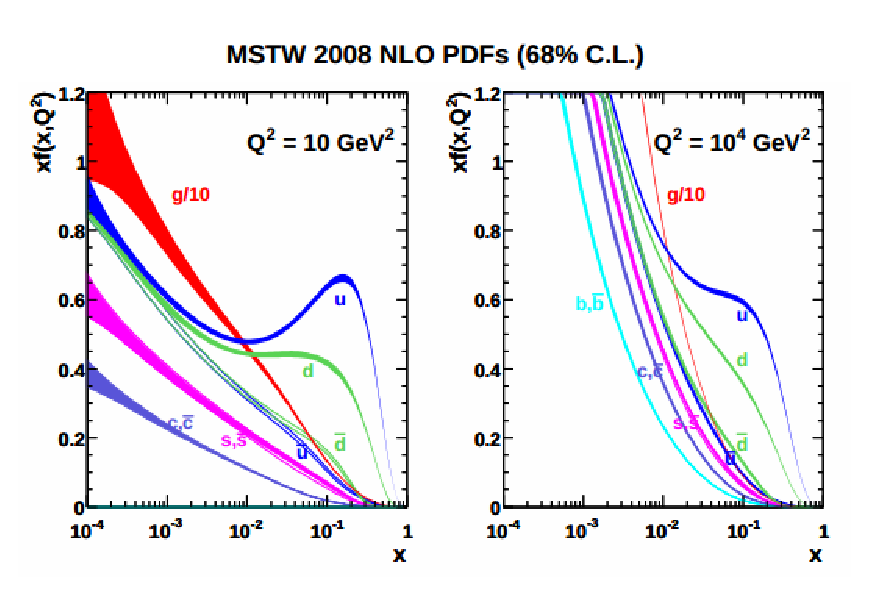
\includegraphics[width=0.75\textwidth]{montecarlo/figures/pdfs2.eps}
}
\caption{Proton PDF functions at transfer momentum
 Q$^2$=10$~$GeV (Q$^2$=10000$~$GeV) on the left (right)~\cite{Martin:2009iq}.\label{fig:PDFs}}
\end{center}
\end{figure}



\subsection{Factorization theorem}\label{sec:factorization}

To treat infinities arising from divergent contributions in loop diagrams,
an arbitrary renormalization scale $\mu_R$ is to be introduced. As a consequence
from requiring that the physical observables be independent from the choice of $\mu_R$,
the strong coupling constant $\alphas$ does depend on the energy scale at which the 
coupling is observed and is, at the leading order:

\begin{equation}\label{eq:alphas}
\alphas(\mu^2) = \dfrac{\alphas(\mu_R^2)}{1 + (11 - \frac{2}{3}n_f)\frac{\alphas(\mu_R^2)}{2\pi}\ln\frac{\mu^2}{\mu_R^2} }, 
\end{equation}
with $n_f$ being the number of quark flavors of the theory and $\mu$ the energy at which we observe the process.

This means that the coupling $\alphas$ decreases with increasing energy scale (small distances)
as a consequence from the factor $11 - \frac{2}{3}n_f$ (the number 11 coming from the self interaction of gluons)
being positive in the theory with $n_f = 6$,
while it increases at lower energies (high distances). These two properties goes under the name of
{\it asymptotic freedom} and {\it confinement} respectively: at low \alphas\ quarks and gluons interact very weakly with 
each other and it is possible to use perturbation theory and the parton model~\cite{Feynman:1969ej}, 
which treats partons as free and non-interacting; when \alphas\ is large instead, partons tend to bound together
into colorless hadrons, predictions from perturbative calculations become less reliable and soft QCD interactions
are typically modeled using tunings from experimental data.

The {\it factorization theorem}~\cite{Campbell:2006wx} allows us to separate the 
two components to compute the cross section as a product of probability functions with
the short distance cross section $\hat{\sigma}_{\rm ab}$ computable in perturbation
theory (pQCD, from perturbatve QCD) as a power expansion of the strong coupling constant $\alphas(\mu_R)$:

\begin{equation}
\begin{split}
  \sigma_{{\rm pp}\to{\rm X}}
  & = \sum_{a,b}%~\in~{\rm partons}}
  \int_{0}^{1}{\rm d}x_a{\rm d}x_b
  ~ f_a(x_a,\mu_{F}) f_b(x_b,\mu_{F})
  \hat{\sigma}_{\rm ab}(x_ap_a, x_bp_b,\mu_R,\mu_{F}) \\
  & = \sum_{a,b}%~\in~{\rm partons}}
  \int_{0}^{1}{\rm d}x_a{\rm d}x_b
  ~ f_a(x_a,\mu_{F}) f_b(x_b,\mu_{F})
  \times {\left[ \hat{\sigma}_{0}(\hat{s}) + \alpha_{S}(\mu_{R}^{2})\hat{\sigma}_{1}(\hat{s},\mu_{F}^{2}) + \dots \right]}. \\
\end{split}
\label{eq:QCDCrossSection}
\end{equation}

Here, $f_i$ ($i=a,b$) are the standard PDFs for partons $a,b = \{g,u,\bar{u},d,...\}$ carrying fractions $x_a,x_b$ 
of the proton longitudinal momentum, and $\sigma_{{\rm pp}\to{\rm X}}$ is the partonic scattering cross-section 
calculated in fixed-order perturbation theory. The $\mu_{F}$ coefficient is newly introduced {\it factorization scale}, 
$\mu_{R}$ is the renormalization scale for the QCD running coupling. Figure~\ref{fig:hardscatter} shows a pictorial
representation of the generic p-p process.

%which can be thought of as the scale that separates the long and short-distance physics, and $\mu_{R}$ is the renormalization scale for the QCD running coupling. Formally, the cross-section calculated to all orders in perturbation theory is invariant under changes in these parameters, but in practice it is not possible to dispose  of a complete set of higher order corrections. It is then necessary to make a specific choice   for the two scales in order to make cross-section predictions. The usual prescription consists in choosing a central value $\mu_R$ for both scales equal to some sensible energy scale in the process (e.g. \mH for Higgs boson production, \mZ for Drell-Yan events, etc.). A range of variation of the renormalization and factorization scales of $\mu_R/2 \le \mu_{R},\mu_{F} \le 2\cdot\mu_R$ is used to determine the uncertainty in the cross-section calculation due to missing higher-order QCD radiative corrections.

\begin{figure}[hbt]\begin{center}
        \myskip\begin{fmffile}{fmfhardscatter}
\unitlength=1mm
  \begin{center}
  \begin{fmfgraph*}(80,45)
    \fmfleft{P1,P2} \fmfright{P11,vv,P22}
    \fmf{fermion,tension=1,lab=$p_b$}{P1,g1}
    \fmf{fermion,tension=1,lab=$p_a$}{P2,g2}
    \fmfblob{.08w}{g1}
    \fmfblob{.08w}{g2}
    \fmf{plain,lab.side=left,lab=$x_bp_b$}{g1,v}
    \fmf{plain,lab.side=left,lab=$x_ap_a$}{v,g2}
    \fmf{dashes}{v,vv}
    \fmf{fermion}{g1,P11}
    \fmf{fermion}{g2,P22}
    \fmfv{lab.dist=.02w,lab=p}{P1}
    \fmfv{lab.dist=.02w,lab=p}{P2}
    \fmfv{lab.dist=.06w,lab.side=left,lab=$f_b(x_b)$}{g1}
    \fmfv{lab.dist=.06w,lab.side=left,lab=$f_a(x_a)$}{g2}
    \fmfv{decor.shape=circle,decor.filled=empty, decor.size=0.20w,lab.side=left,lab.dist=-0.09w,lab=$\hat{\sigma}(x_ax_bs)$}{v}
    \fmfv{lab=X}{vv}
    \fmffreeze
    \renewcommand{\P}[3]{\fmfi{plain}{%
        vpath(__#1,__#2) shifted (thick*(#3))}}
    \P{P1}{g1}{0,1}  \P{P1}{g1}{0,-1}
    \P{P2}{g2}{0,1}  \P{P2}{g2}{0,-1}
    \P{g1}{P11}{0,1} \P{g1}{P11}{0,-1}
    \P{g2}{P22}{0,1} \P{g2}{P22}{0,-1}
  \end{fmfgraph*}
  \end{center}
\end{fmffile}
\myskip
  	%\includegraphics[width=0.5\textwidth]{montecarlo/figures/fmfhardscatter}}
	\caption{Diagram of a generic hard scattering process. The partons, extracted from the colliding p-p pair,
  carry a momentum fraction with respect to the proton energy described by a parton distribution function. 
  The scattering of the partons is computed perturbatively and hence the kinematic properties of the final state object $X$ are predicted. \label{fig:hardscatter}}
\end{center}\end{figure}
%the {\it parton distribution functions} (PDFs)
%distribution functions (PDFs), describing the probability to
%extract a quark or gluon from the protons in the initial state,
%a perturbative cross-section for the hard scattering, 
%and a probabilistic description of the final state by a parton
%shower Monte Carlo. 

Equation~\ref{eq:QCDCrossSection} refers to a sum of final state and is, therefore, inclusive. The choice for the 
renormalization and factorization scale values is usually to take them of the order of some typical hard scale 
entering the process like, e.g., the mass of the top quark for top-anti-top pair production.
The cross section calculations are done in pQCD are in general either provided at Leading Order (LO) 
or at Next-to-LO (NLO). NLO calculations include corrections from virtual exchange or emission of a massless parton.


\section{Simulation of p-p collisions}\label{sec:MCsimulation}

The most interesting phenomena under study are scattering events with 
large momentum transfer or with production of massive particles, also
called ``hard scattering'' events.
Typical pQCD calculations can only provide an inclusive description of
the process, while Monte Carlo programs give an exclusive picture
of the event. 
A p-p collision event in Monte Carlo simulation
is the combination of different sub-processes,
illustrated in Figure~\ref{fig:collision}: %The core of the event, the hard interaction, produces a scattering at large angle of the colliding partons or new particles. 
%Generally speaking, Monte Carlo simulation is a
%mixture of various components: 
it comes with a large library of
Standard Model and Beyond Standard Model cross section from which the
hard scattering process is chosen; it has a showering algorithm to 
generate the dominant pQCD effects, adding the emission of colored partons
to the hard process enhanced with collinear and soft singularities;
it implements hadronization for the high energy partons of the final
state; it describes the underlying event according to some phenomenological
model; it includes libraries for the weak decay of unstable hadrons.

A set of drawings in Figure~\ref{fig:eventevolution} shows the sequence
of the evolution of Monte Carlo event simulation, starting from the
plain hard scatter and adding step by step the other components.

%~\cite{Mangano:933464}
%Some generators instead describe ``multi-leg'' processes (with multiple final state partons)  with LO matrix elements for each parton multiplicity (see below). In order to take into account higher order corrections, MC simulations use the pQCD  predictions at a given order  supplemented by parton shower.  In addition, the MC simulation include non-perturbative effects such as hadronization  (formation of hadrons from partons)  and underlying event (soft interaction between the remnant partons of the colliding hadrons). Figure \ref{fig:collision} shows a sketch of a proton-proton collision as it is described in MC simulations. 

\begin{figure}[tbph]
\begin{center}
\subfigure{
  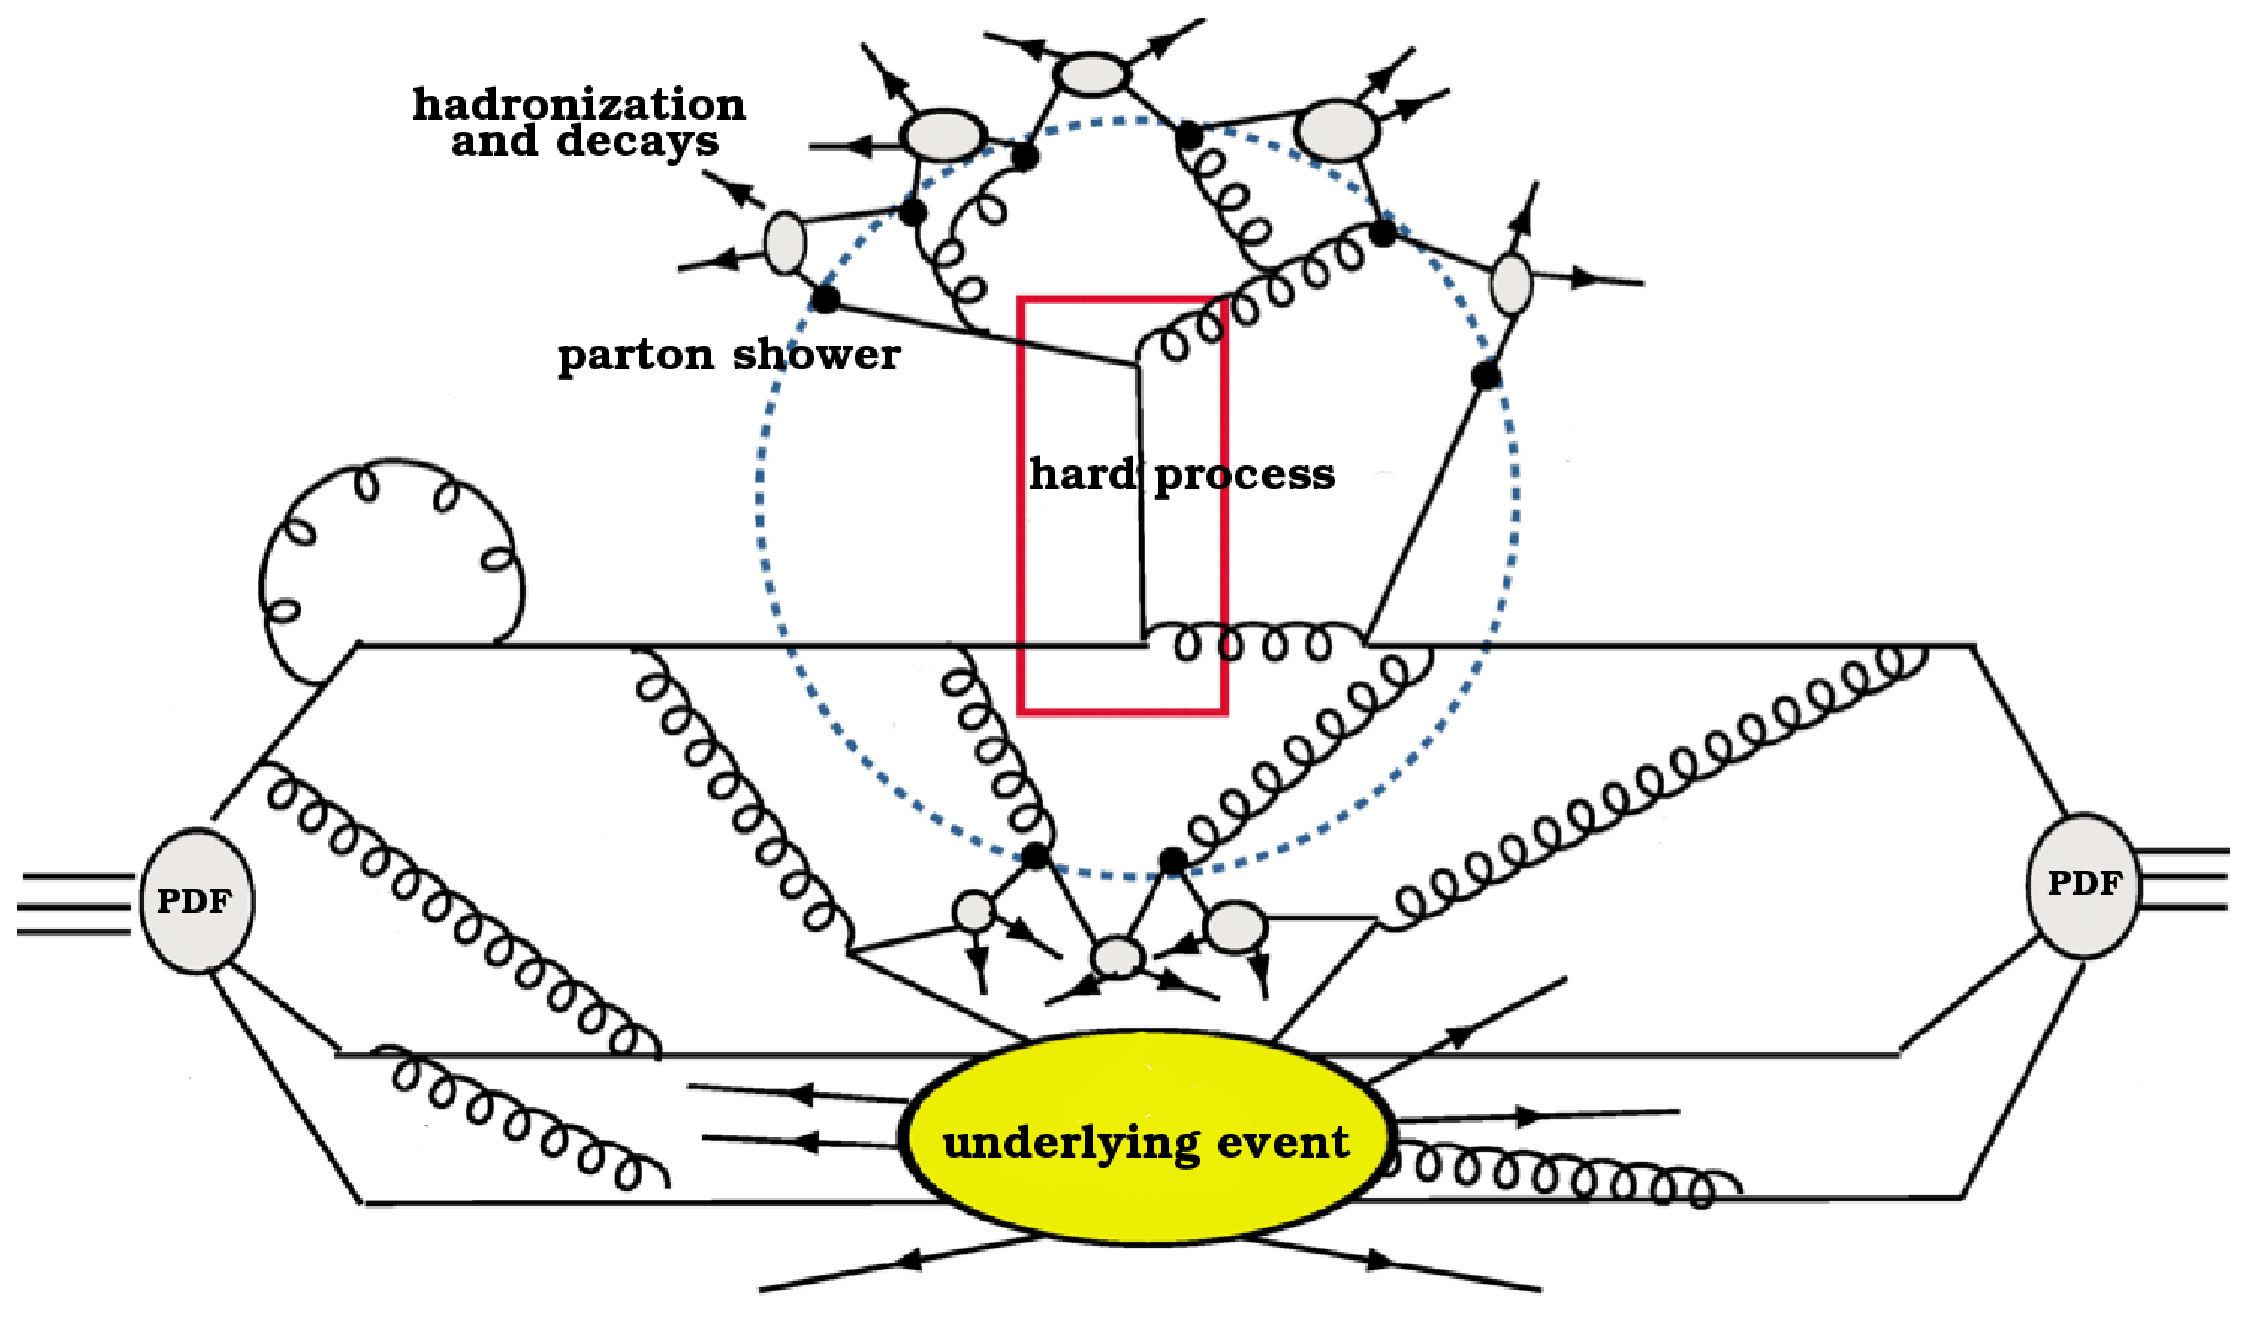
\includegraphics[width=0.8\textwidth]{montecarlo/figures/my_collision}
}
\caption{Drawing describing a hadron-hadron collision from the Monte Carlo
point of view. Partons from the hadron share its energy according to the PDFs. 
The dotted circle separates pQCD events (hard scattering 
and initial and final state radiation) from non-perturbative effects (parton shower, 
hadronization, initial emissions included in the PDFs, and underlying event)\cite{Mangano:933464}.\label{fig:collision}}
%\end{center}
%\end{figure}
%\begin{figure}[htb]\begin{center}
	\subfigure[]{\label{fig:event2}
  	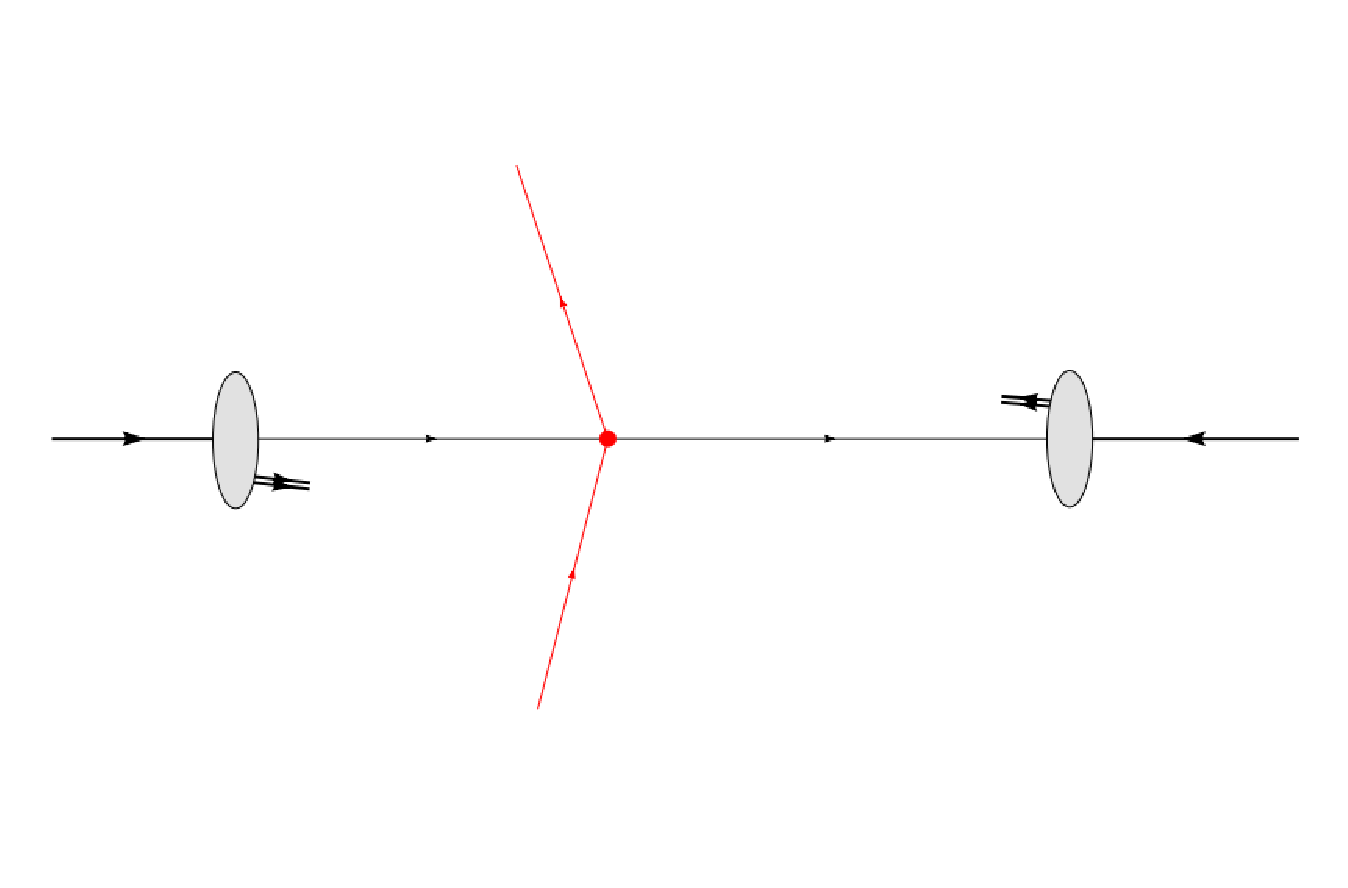
\includegraphics[width=0.45\textwidth,height=0.25\textwidth]{montecarlo/figures/event2}}
	\subfigure[]{\label{fig:event3}
  	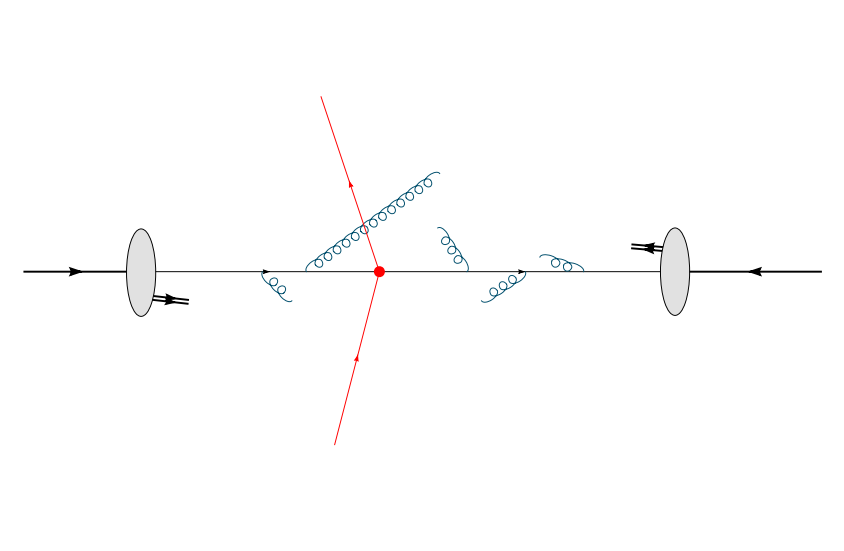
\includegraphics[width=0.45\textwidth,height=0.25\textwidth]{montecarlo/figures/event3}}\\
	\subfigure[]{\label{fig:event4}
  	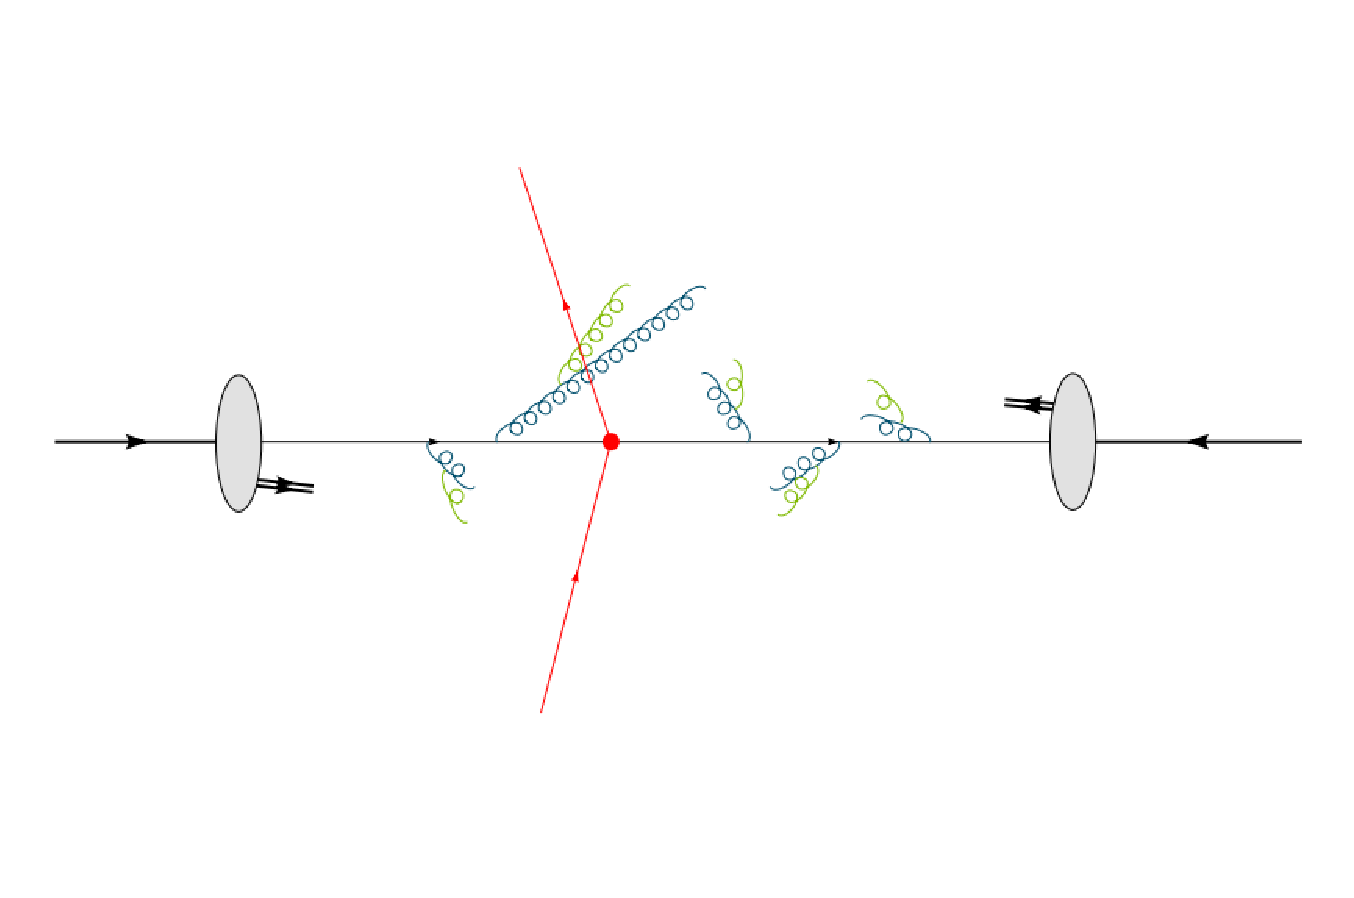
\includegraphics[width=0.45\textwidth,height=0.25\textwidth]{montecarlo/figures/event4}}
	\subfigure[]{\label{fig:event5}
  	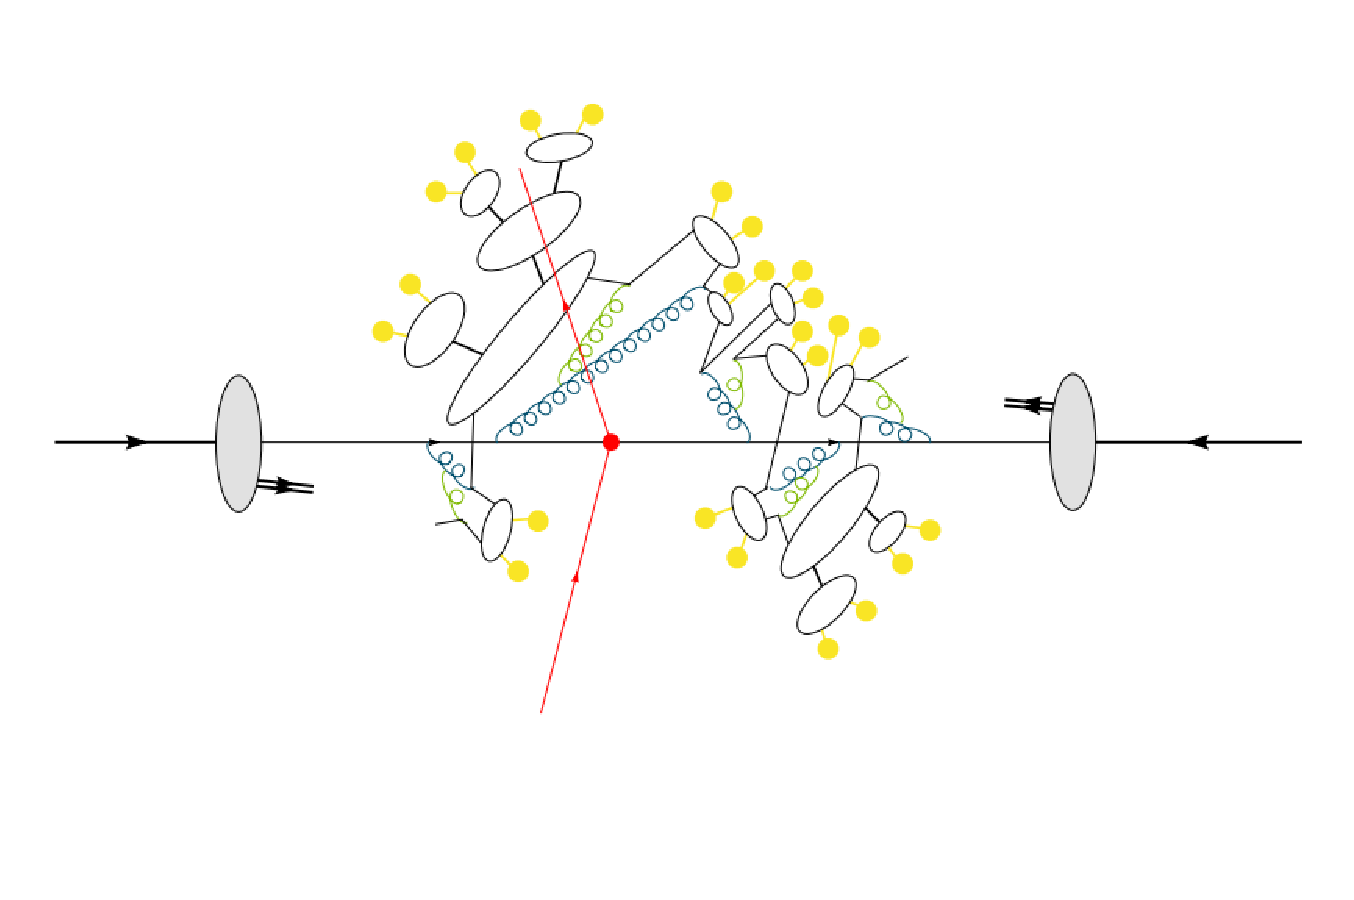
\includegraphics[width=0.45\textwidth,height=0.25\textwidth]{montecarlo/figures/event5}}\\
	\subfigure[]{\label{fig:event6}
  	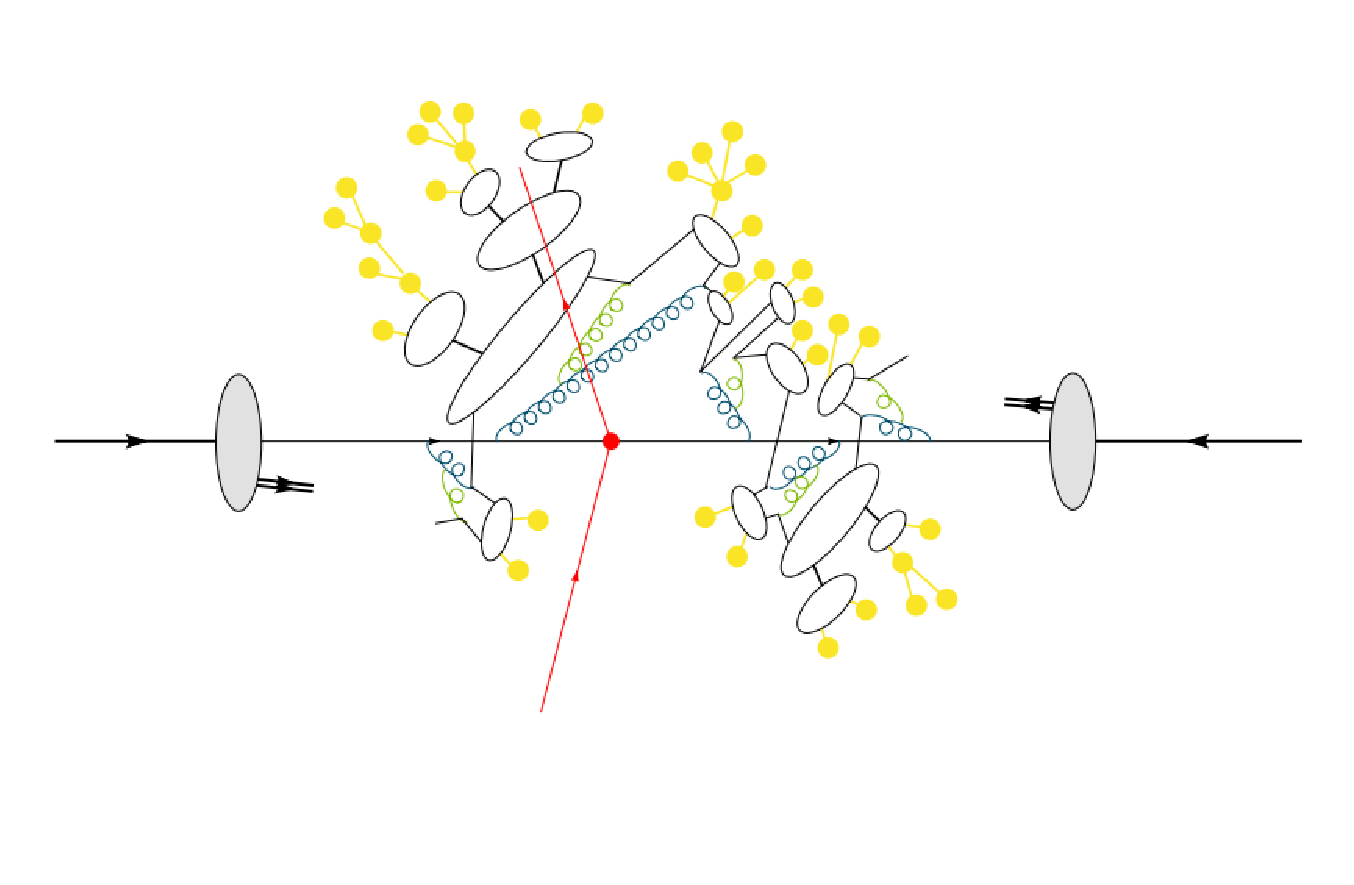
\includegraphics[width=0.45\textwidth,height=0.25\textwidth]{montecarlo/figures/event6}}
	\subfigure[]{\label{fig:event7}
  	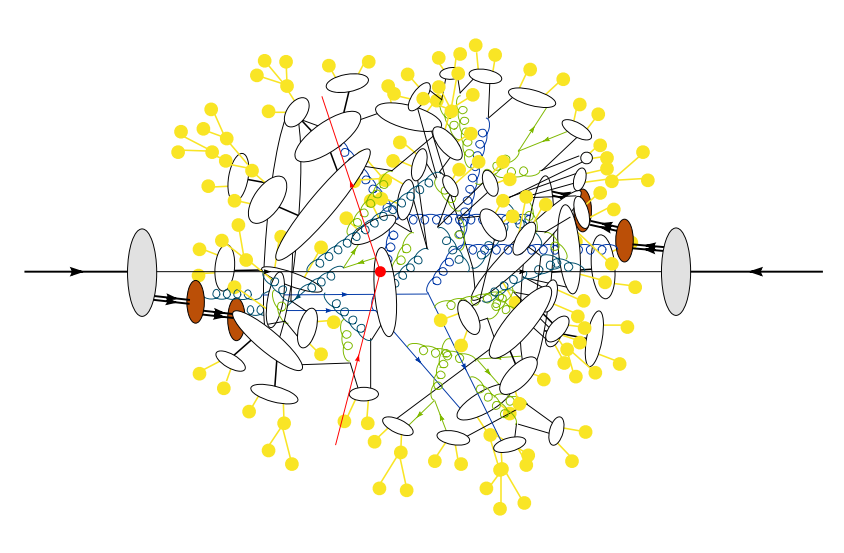
\includegraphics[width=0.45\textwidth,height=0.25\textwidth]{montecarlo/figures/event7}}
	\caption{Set of frames of Monte Carlo event generation evolution: (a) hard scattering of two
        partons; (b) and (c) parton showering; (d) hadronization; (e) final particle decays; (f)
        underlying event simulation. Drawings from~\cite{Gieseke}.\label{fig:eventevolution}}%\footnotemark.}
\end{center}\end{figure}

%\footnotetext{Taken from the slides: \url{http://th-workshop2009.desy.de/e59393/e59379/infoboxContent59381/Gieseke.pdf}.}


\subsection{Hard interaction}\label{sec:matrixelement}

Recalling what discussed in Section~\ref{sec:factorization} about the computation in pQCD
of the hard scattering cross section of a typical LHC $pp\to X$ event, we can rewrite
Equation~\ref{eq:QCDCrossSection} as:
\begin{equation}
\begin{split}
  \sigma_{{\rm pp}\to{\rm X}}
  & = \sum_{a,b}%~\in~{\rm partons}}
  \int{\rm d}x_a{\rm d}x_b
  ~ \int
  ~ f_a(x_a,\mu_{F}) f_b(x_b,\mu_{F})
  {\rm d}\hat{\sigma}_{\rm ab}(x_ap_a, x_bp_b,\mu_R,\mu_{F}) \\
  & = \sum_{a,b}%~\in~{\rm partons}}
  \int{\rm d}x_a{\rm d}x_b
  ~ \int{\rm d}\Phi_{\rm X}
  ~ f_a(x_a,\mu_{F}) f_b(x_b,\mu_{F})
  ~ \times \dfrac{1}{2x_ax_bs}\big|\mathcal{M}_{\rm ab}\big|^2(\Phi_{\rm X},\mu_R,\mu_{F}),  \\
\end{split}
\label{eq:matrixelement1}
\end{equation}
where we introduced the dependence on the final state phase space $\Phi_{\rm X}$, the parton flux
$\frac{1}{2x_ax_bs}$ (with $s$ being the \cme\ squared) and the {\it matrix element} $\mathcal{M}_{\rm ab}$,
which is also written as a sum over Feynman diagrams:
\begin{equation}\label{eq:matrixelement2}
\mathcal{M}_{\rm ab} = \sum_i \mathcal{F}^{(i)}_{\rm ab}.
\end{equation}

%presence of collinear and soft divergences in fixed order calculations with a definite final state. Only by summing over different final states these divergences can cancel, thereby allowing the computation of certain (i.e. the collinear and infrared insensitive) inclusive quantities. The only frameworks in which exclusive quantities can be computed must involve the resummation of an infinite class of Feynman graphs. 



\subsection{Parton shower}\label{sec:partonshower}

Parton shower adds higher order corrections to the hard scatter using an approximation scheme,
since real radiative corrections to any inclusive quantity (like the hard cross section as computed at
fixed order in pQCD) are divergent. The dominant contributions below a cut-off parameter, associated to 
collinear parton splitting or soft gluon emission, are included iteratively ordered in sequence of, typically, smaller emission angles.
%The Kinoshita-Lee-Nauemberg theorem assures that virtual corrections cancel.

There are three possible processes for QCD emission: 
$q\to gq$, $g\to gg$ and $g\to q\bar{q}$.
The cross section then factorizes into the product of 
the parent parton production cross section times
 a splitting factor. Considering e.g. the $q\to gq$ 
splitting from a tree level process with $n+1$
final state particles we can graphically represent it as
in Figure~\ref{fig:factorization}, with the quark $k$ and the
gluon $l$ being emitted at a small angle $\theta$.
Mathematically we have:
\begin{equation}
  \big|\mathcal{M}_{n+1}\big|^2{\rm d}\Phi_{n+1} \to 
  \big|\mathcal{M}_{n}\big|^2{\rm d}\Phi_{n} \dfrac{\alphas}{2\pi}\dfrac{{\rm d}t}{t}P_{q,qg}(z)\dfrac{{\rm d}\phi}{2\pi},
\label{eq:splitting1}
\end{equation}
where $\phi$ is the azimuth defined by $\vec{k}$ and$\vec{l}$ around the $\vec{k+l}$
direction, $z$ is an arbitrary parameter in general defined as a ratio between the
energy of the particles emitted:
\begin{equation}
  \label{eq:zfromk0} z = \frac{k^0}{k^0 + l^0},
\end{equation}
and $t$ is the {\it hardness} parameter characterizing the divergence
and the ordering of the splittings. It has the dimensions of a mass, and 
the preference is to take it as $t = E^2\theta^2$. 
The values for $\phi$, $z$ and $t$ are generated randomly during the Monte
Carlo simulation process. 
The function $P_{q,qg}(z)$ is
the Altarelli-Parisi splitting function, and is the only term that changes in
Equation~\ref{eq:splitting1} between $q\to gq$, $g\to gg$ and $g\to q\bar{q}$ 
splittings.

\begin{figure}[hbt]\begin{center}
	\subfigure[]{\label{fig:factorization}
  	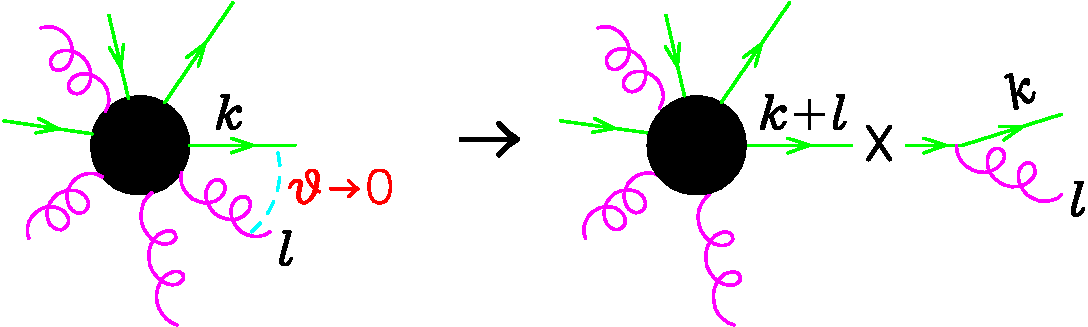
\includegraphics[width=0.45\textwidth]{montecarlo/figures/factorization}}\hskip5ex
	\subfigure[]{\label{fig:splitkin}
  	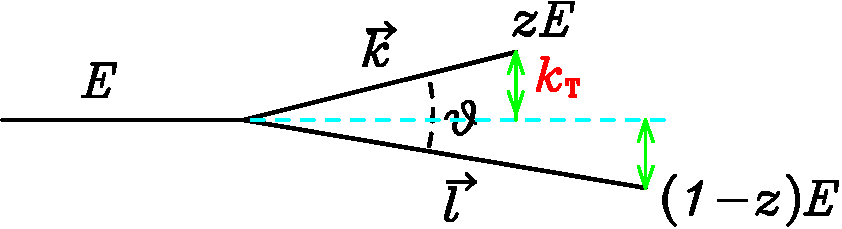
\includegraphics[width=0.4\textwidth]{montecarlo/figures/splitkin}}
	\caption{Left: graphical representation of the $q\to qg$ splitting. The
        black circles represent the $\mathcal{M}_{n+1}$ and $\mathcal{M}_{n}$
        amplitudes of the tree-level processes. Right: kinematic of the splitting~\cite{Ambroglini:2009nz}.}
\end{center}\end{figure}

Factorization holds if the virtuality of the splitting parton $q^2 = (k+l)^2$ 
is negligible with respect to the energies entering the process, and 
can be applied iteratively as shown graphically in Figure~\ref{fig:factorization2}.
At this point, allowing for $n$ splitting processes, the cross section can be written as:
\begin{equation}
  \label{eq:leadinglog} 
  %\sigma_0 \alpha_S^n \int \frac{d t_1}{t_1}  \frac{d  t_2}{t_2} \ldots \frac{d t_n}{t_n} \times \theta (Q^2 > t_1 > t_2 > \ldots >  t_n > \lambda^2) = 
  \sigma_0 \frac{1}{n!} \alpha_S^n \log^n
  \frac{Q^2}{\lambda^2},
\end{equation}
where $Q$ is the upper cut-off scale called {\it annihilation energy} that determines
when the showering starts, and $\lambda$ is the infrared cut-off. The shower ends
when the virtuality $q^2$ reaches the {\it hadronization scale}, which is of the
order of $1~\gev^2$. From the cross section expression of Equation~\ref{eq:leadinglog},
this procedure is called ``leading log approximation''.

\begin{figure}[tb]\begin{center}
	\subfigure{
  	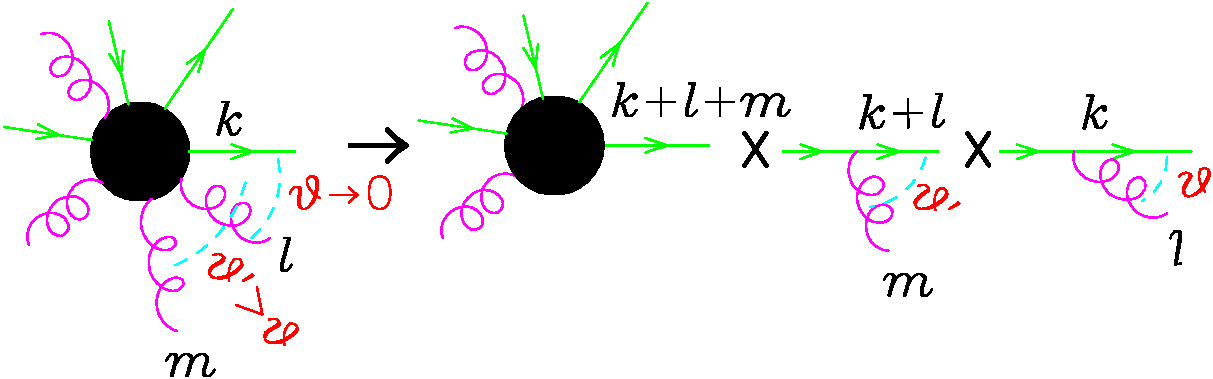
\includegraphics[width=0.6\textwidth]{montecarlo/figures/factorization2}}
	\caption{Recursive application of factorization, with the angles ordered
        as  $\theta' \gg \theta \rightarrow 0$~\cite{Ambroglini:2009nz}.\label{fig:factorization2}}
\end{center}\end{figure}

Once the shower is developed, the vertices and lines of the final configuration are
assigned weights, which are for each vertex:
  \begin{equation}
    \label{eq:splitvert} \theta (t - t_0) \hspace{0.75em} \frac{\alpha_S
    (t)}{2 \pi} \hspace{0.25em} \frac{dt}{t} \hspace{0.25em} P_{i, j l} (z)
    \hspace{0.25em} dz \hspace{0.25em} \frac{d \phi}{2 \pi},
  \end{equation}
and for each line are the so-called {\it Sudakov form factors}:
  \begin{equation}
    \label{eq:sudadef} \Delta_i (t', t'') = \exp \left[ - \sum_{(j l)}
    \int_{t''}^{t'} \frac{dt}{t} \int_0^1 d z \hspace{0.75em} \frac{\alpha_S
    (t)}{2 \pi} \hspace{0.25em} \hspace{0.25em} P_{i, j l} (z) \right]
  \end{equation}
where $t'$ is the value of $t$ at the upstream vertex, and $t''$ 
at the downstream vertex. If we reached the end of the graph,
$t''$ is substituted by a cut-off $t_0$.
The Sudakov form factors specify the range of the $z$ parameter for 
which the splitting is resolvable and represent the probability
of {\it not} splitting. Figure~\ref{fig:showergraph} shows
the typical graph shape of a shower evolved with splittings
strongly ordered in angle.

\begin{figure}[hbt]\begin{center}
	\subfigure{
  	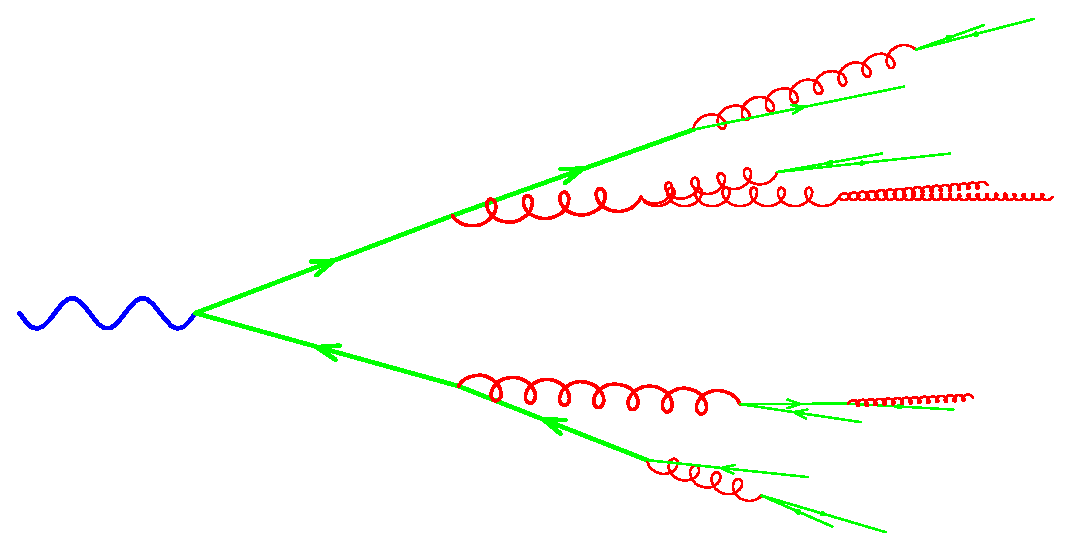
\includegraphics[width=0.6\textwidth]{montecarlo/figures/MCWSShower}}
	\caption{An example of a typical shower final graph~\cite{Ambroglini:2009nz}.\label{fig:showergraph}}
\end{center}\end{figure}

\subsubsection{Initial and final state radiation}\label{sec:isrfsr}

We discussed up to now the development of parton shower arising
from the emission from hadrons produced in the hard scattering, i.e. 
starting in general at an high annihilation scale $Q^2$ and progressively
reaching the hadronization scale. This process goes under the name of
{\it final state radiation} (FSR), as it is generated from outgoing
partons of the hard interaction.

Parton shower can of course also happen before the hard interaction, and
is called {\it initial state radiation} (ISR) as the incoming partons
of the hard scattering originate the emission. In this case
there is an important difference in the shower evolution, that is
that the final energy of the showering is the hard interaction energy
scale. To respect this fact, Monte Carlo simulation of ISR adopts a 
``backward evolution'', first setting the correct parton momentum distributions
for the hard scatter, and then developing the shower backward, with the 
intermediate partons aquiring energy at each emission. The Sudakov form 
factors are then slightly different from Equation~\ref{eq:sudadef}, being
rescaled by a factor that takes into account the PDFs of the parton at the
two vertices.


\subsubsection{Matrix element and parton shower matching}\label{sec:matching}

\subsection{Hadronization}\label{sec:hadronization}

When partons reach the hadronization scale energy $Q\sim 1\gev$ after showering,
they recombine in bound colorless states according to the confinement
principle, holding at low momentum. The so-called {\it parton-hadron duality}
assumes that no high momentum transfer is needed in the recombination,
as it happens  close in phase space. This is a property of QCD
experimentally observed, but there are no theoretical arguments
explaining the hadronization. The solution is then to rely on
phenomenological models.

The principle at the basis of hadronization models used in Monte Carlo is the 
{\it large $N_c$ limit}, or {\it planar limit}, where $N_c$ is the number
of colors and we consider the QCD value $N_c = 3$ as just the dominant
contribution. Simple rules are then defined: color and anticolor indices
go from 1 to $N_c$; quark and antiquark lines are oriented and assigned
a color and anticolor index respectively; gluon lines are oriented and assigned
a pair of color-anticolor indices to achieve color neutrality. 
The color structure of the three splitting
processes according to these rules are shown in Figure~\ref{fig:planarrules}.
While the assignment of color connections in the case of $q\to qg$ and
$g\to q\bar{q}$ splittings is univocal, for $g\to gg$ there are two possible
configurations (where by inverting the two final state gluons transform one
into the other) and when the color connections are reconstructed they are chosen
with a 50\% probability each. The final picture looks e.g. like the graph
in Figure~\ref{fig:colourflow}, where the important information is not the
specific color assigned to the final state parton, but rather the {\it color flow}.


\begin{figure}[hbt]\begin{center}
	\subfigure[]{\label{fig:planarrules}
  	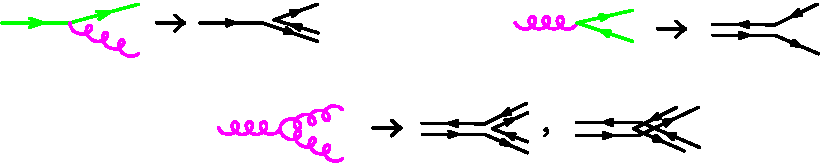
\includegraphics[width=0.45\textwidth, height=0.18\textwidth]{montecarlo/figures/planarrules}}\hskip5ex
	\subfigure[]{\label{fig:colourflow}
  	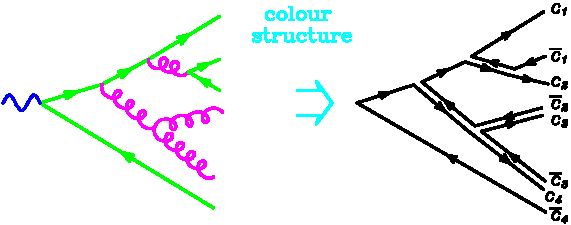
\includegraphics[width=0.45\textwidth]{montecarlo/figures/colour2}}
	\caption{Left: rules to assign color connections in the splittings
        $q\to qg$ (top left), $g\to q\bar{q}$ (top right) and $g\to gg$ 
        (bottom). Right: example of a color connected shower~\cite{Ambroglini:2009nz}.}
\end{center}\end{figure}

At this point, two possible phenomenological fragmentation models come in the game
to bound partons into hadrons starting from the color connected final state.
They both have been tuned using collider measurements over the last decades
to properly describe the final state hadron multiplicity and need in general
a large number of parameters.

The first hadronization scheme is called {\it Lund string model} and ties a quark
with an antiquark plus a number of intermediate gluons, like
stretching a string (or a ``color flux tube'') from the quark
to its color-connected antiquark taking in the gluons that
lie inbetween them. This can be see as an illustration in 
Figure~\ref{fig:had_colorflow} and Figure~\ref{fig:had_string}:
the first string collects the quark with color $c_1$, the antiquark
with color $\bar{c}_4$ and all the final state gluons along the path.
 uses string dynamics to describe the color flux between quarks. 
In other words, the string between the quark and antiquark produces a linear
confinement potential.

The other hadronization scheme is the {\it cluster model}, where
final state gluons are forced to split into a quark-antiquark pair
and then color connected quark-antiquark pairs are bounded together.
Figure~\ref{fig:had_cluster} presents a graphical illustration of the
concept. Because of {\it preconfinement} (the fact that color connected pairs
with large invariant masses are Sudakov suppressed in angular ordered showers)
the cluster can be associated with an hadronic two-body system. 

During the last decades, different measurements at colliders have
been used to tune these models to properly describe 
the hadron multiplicity in the final state.


\begin{figure}[hbt]\begin{center}
	\subfigure[]{\label{fig:had_colorflow}
\def\svgwidth{0.3\textwidth}
\input{montecarlo/figures/had_colorflow.eps_tex}}
	\subfigure[]{\label{fig:had_string}
  	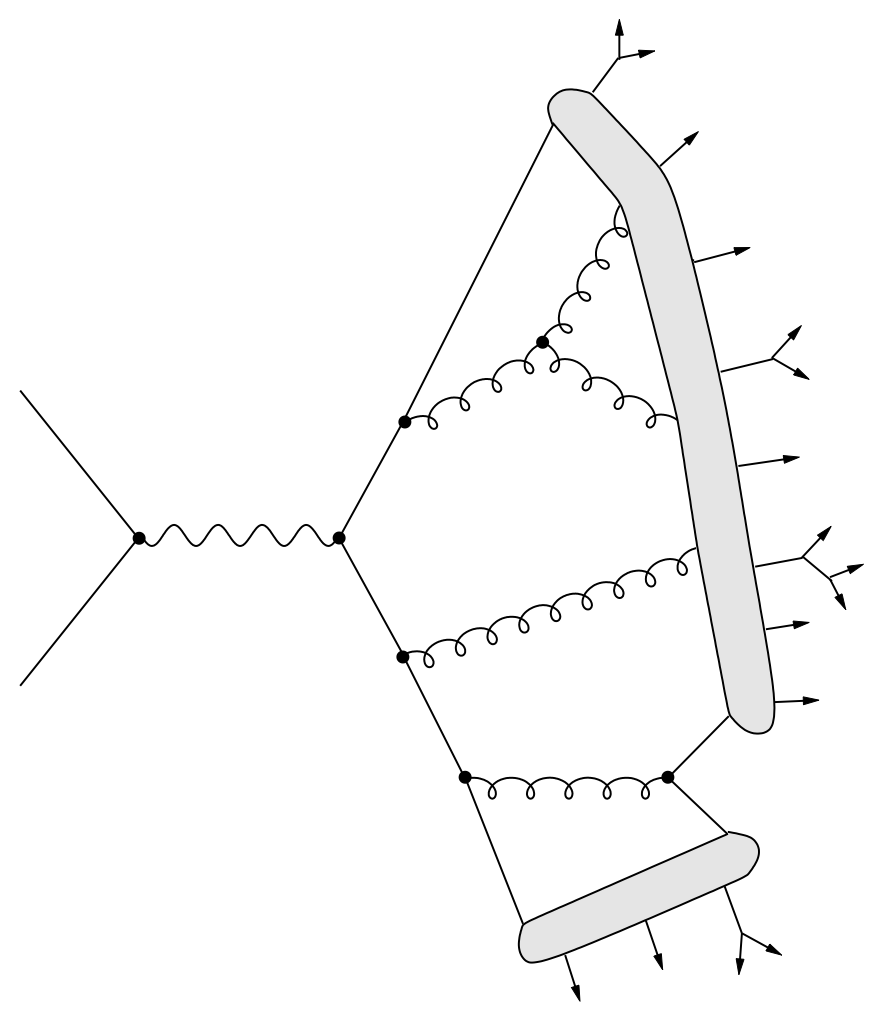
\includegraphics[width=0.3\textwidth]{montecarlo/figures/had_string}}
	\subfigure[]{\label{fig:had_cluster}
  	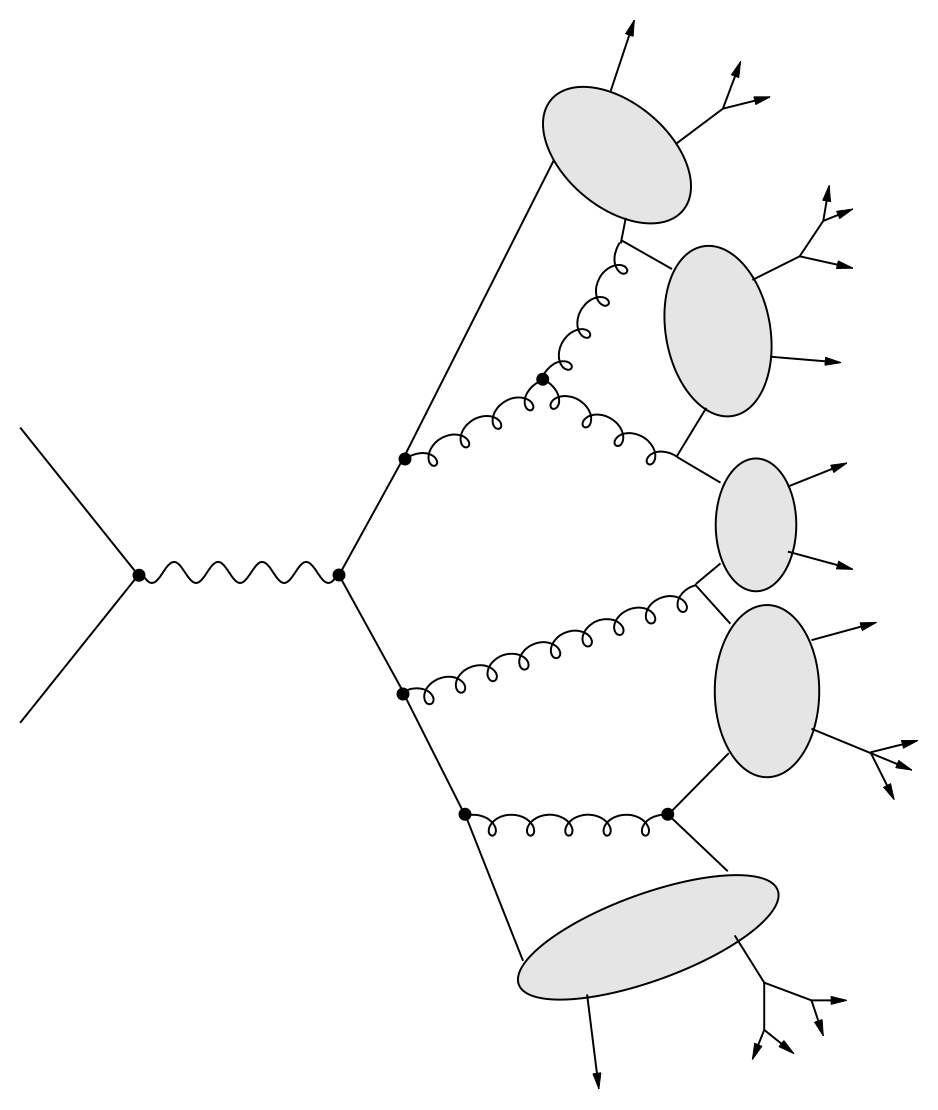
\includegraphics[width=0.3\textwidth]{montecarlo/figures/had_cluster}}
	\caption{Drawing of a color connected parton shower graph (a) completed with hadronization from the Lund string model (b) and the cluster model (c)~\cite{Mangano:933464}.}
\end{center}\end{figure}



\subsection{Underlying event}\label{sec:underlyingevent}

With ``underlying event'' (UE) we refer to the secondary parton interactions 
at low transfered momentum that accompany the main hard process. 
The underlying event is flavor- and color-connected to the hard scattering
and in real data is in general not separable from the event of interest.
It is typically observed as jets of particles close to the direction
of the beam and cannot be modeled with perturbative QCD but is instead
studied from experimental data on {\it minimum bias} events at low
momentum.

\section{Generators}\label{sec:generators}

\section{ATLAS simulation}\label{sec:MCdetector}
